\documentclass{article}
\usepackage{a4, fullpage}
\usepackage{float}
\usepackage{amssymb,amsmath}
\usepackage[T1]{fontenc}
\usepackage{graphicx}
\usepackage{multicol}
\usepackage{alltt}

\begin{document}

%-------------------------------------------------------------------------------
%    TITLE PAGE
%-------------------------------------------------------------------------------

\begin{titlepage}
\newcommand{\HRule}{\rule{\linewidth}{0.5mm}}
\center
\textsc{\LARGE Imperial College London}  \\[1.5cm]
\textsc{\Large Department of Computing}  \\[0.5cm]
\textsc{\large Course 350: Management and Business for Computing Engineers} \\[0.5cm]

\HRule \\[0.6cm]
{\huge \bfseries name of company here} \\[0.3cm]
\HRule \\[1.5cm]

\begin{minipage}{0.4\textwidth}

% author
\begin{flushleft} \large \emph{Authors:} \\
Alina     \textsc{Boghiu}    \\
Giovanni  \textsc{Charles}   \\
Adam      \textsc{Fiksen}    \\
Sahil     \textsc{Jain}      \\
\L ukasz  \textsc{Koprowski} \\
Rutwik    \textsc{Shah}      \\
John      \textsc{Walker}    \\
\end{flushleft}

% supervisors
\end{minipage}~
\begin{minipage}{0.4\textwidth}

\begin{flushright} \large \emph{Lecturer:} \\
Nick \textsc{Coutts}
\end{flushright}


\end{minipage}\\[4cm]


\includegraphics[width=\textwidth]{apples.jpg}

\end{titlepage}

%-------------------------------------------------------------------------------

\section{Executive summary}

business model = product (disguised as service for legal reasons - absolut?)

business objective
maximise sales
 - new to the market
   explain the required infrastructure to sell a lot

\section{Vision statement}

Our mission is to bring a mid priced cider to the people of India. India
has the second largest population in the world, and has an estimated market size
of 500 million alcohol consumers [better estimate]. At the moment, there is one
provider of cider in India, and we would like the change that.

We want to be a brewery. We will brew our own cider in the state of Himachal
Pradesh, which is the source of the majority of the apples in India. Along with
producing cider, we will sponsor other exclusive bars and clubs.

Operating in India which is well known for its corruption, we want to practice
ethical development. eg corrupt free, no bribes, no blood cider forced labour
fairtrade

We hope to gain popularity in major establishments, in Delhi and Mumbai through
the open minded youth and bar owners.

Our cider will become a desired commodity through exclusivity and we will be
able to research our market further at this point with minimal risk.

We will adapt and pick up popularity and scale up to make it available to the
public.

%please discuss even if you do not think it is an issue
Operating in India which is well known for its corruption, we want to practice
ethical development. eg corrupt free, no bribes, no blood cider forced labour
fairtrade

ethics.
fairtrade - look at poverty + with partners
poverty - provide jobs and food to the villagers. improve infrastructure (added benefits - tax exemptions)
religion - no issue, alcohol is still sold across all of india
corruption - no bribes, do everything by the books
age restriction - different restrictions for different states, alcohol content
health - people already drink, we arent trying to get more people to drink, just introduce it to current drinkers
eco(water recycling, using up all the apples) - recycle apple waste. recycle all water. solar energy. supply of apples
%add as you please

type = pvt. ltd. co. - control of the company

\section{Management team}

\section{Introduction to the market}
\section{Products and services offered}
\section{Marketing plan}

\subsection{Route to Market}
\subsubsection{Be At One}
B@1 was founded from the ashes of an Indian restaurant in Battersea park by
three experienced bartenders.

They started their bar on £60,000 raised from savings and car loans and after a
year grew to a stage where they could start a second bar.

We believe their success stems from their intimate knowledge of the local drinkers and thier personal service to create a great night for each customer.

\subsubsection{Red Bull}
Dietrich Mateschitz attempted to introduce an existing Thai drink, a favourite
for local truck drivers, to a western market, an objective which
mirrors our own.

After initial market research he was strongly advised not to continue with his
venture. He continued regardless on the grounds that the research would be
relevant for an existing product but not his new 'energy drink' which was
unheard of at the time.

He then employed a marketing intensive business strategy focused on the high energy activity sector. We believe that this was important in getting people to warm to the new unfamiliar product, and retain its strong market position despite the emerging competitors. 

\subsubsection{New Albion Brewing Company}
This was a small scale venture by optical engineer Jack McAuliffe in California.
He made a brewhouse from scratch able to produce 7.5 barrels of ale a week. His
company became respected by beer enthusiasts and was very popular. However his
brewery could not produce enough volume to survive, was unable to raise
investment to expand and ground to a halt eight years after it opened.

We learn from this that small scale production is not without risk and under supply 
could be detrimental to our growth. In the early stages it would be sensible to
sell at a high markup to give us a good chance of survival.

\subsubsection{Conclusion}
Our proposed route to market begins with the launch of a microbrewery in [city].
This is in order to test manufacture on a small scale and conduct market research for later expansion. A brewpub will allow us to get as close as possible to the consumer and the production process so that we can best understand our customers and quickly react to their response.

This route is cheaper than building a factory since manufacture would be on a
smaller scale. But, as shown from the brewpub market and the B@1 case, a microbrewery is large/profitable enough to be sustainable.

We must ensure that our market research is focused and in depth so that it is
useful for development. This can be achieved by [something].

Brand awareness will be very valuable for the introduction of a new alcoholic
drink. Sponsorship of festivals, fashion shows ... will play a big part in our
company.

We will sell at a top mid tier price to set it apart from other light alcoholic
beverages, as Red Bull and Innocent have done with thier industries. Our product
currently has no alternative and will be sought after so we believe it could support 
a premium price tag. 

After 2-3 years, we hope to have a large brand awareness and to seek investment for
for mass production... 

\subsection{Market Analysis}
\subsubsection{Current Competitors in the Cider Market}
At the moment, there is only one company which produces cider in India.
The company, Green Valley Cider, produces Tempest Cider in the state of Himachal
Pradesh, where they own several acres of apple orchards.

\subsubsection{Current Competitors in the Microbrewery Market}
\begin{itemize}
\item Rockman's Beer Island, Gurgaon - Located in the largest shopping mall in
			 Gurgaon (bordering New Delhi), Rockman's Beer Island was India's first
			 micro pub brewery. They offer four types of beer: Lager Strong Beer, Dark
			 Beer, Lager Beer and Wheat Beer, and they aim to serve some exclusive
 	     flavoured beers by the summer. Along with the micro pub brewery, they also
			 own an exclusive German restaurant and a digital auditorium covering an
	     area of around 3500 m$^2$. Rockman's are planning to expand now by opening
			 their branch in different locations in India.
\item Toit, Bangalore - Located in the Technology capital of India, Toit has been
			 doing really well since it has opened. They offer 6 different types of beers,
			 which are Toit's Basmati Blonde, Tintin Toit, Toit Weiss, Toit Red, Colonial
			 Toit and Toit's Dark Knight. They are currently in the process of introducing
			 exclusive Toit merchandise, along with their wide selection of food and alcohol.
			 Toit are planning on making the branch national by the end of this year.
\item The Biere Club, Bangalore - Another micro pub brewery which is located in
			 Bangalore, The Biere Club also brews around 6 different types of beers, which
			 include Lager, Ale and Wheat. The Biere Club are planning on making
			 partnerships with rich individuals for expansion in the future.
\item Doolally, Pune - Located in Pune, Doolally has been operational for around
			 three years. It is located in a boutique hotel, and plans to open in a few more
			 locations soon.
\end{itemize}

\subsubsection{Conclusion}
As we can see, there is a large market for alcohol in India, who are eager to try
out new things, which can be seen by the successes of these microbreweries. As India
continues to grow to become a bigger powerhouse in the world, it will attract more
foreigners, which means that people who already know about cider and like it
will increase in the country. This increasing market size makes us believe that
cider will become increasingly popular in India once introduced properly.

\section{Advertising}
\subsection{Current Laws Affection Alcohol Advertising}
In the 90s, extensive surveys resulted in the conclusion that liquor advertisements
were directly influencing the consumer's purchasing behaviour, which led to the
introduction to new laws. Ever since the Cable Television Network Amendment Bill
came into effect on September 8$^{th}$ 2000, advertising alcoholic beverages on
television networks and billboards is completely banned in India.

\subsubsection{How the law has affected advertisment}
Although illegal, alcohol companies have found a way to spread their name through
the media by the use of surrogate advertisment. Surrogate Advertisement refers
to the form of advertisement which is used to promote banned producted, which is
alcohol in our case, in the disguise of another product.

Nearly all alcohol brands have now created other products which they use to advertise
their alcohol. Examples of this include Bagpiper Whiskey creating a Club Soda with
their brand name, Royal Stag creating Music CDs and Royal Challenge creating Mineral
Water and Music CDs.

\begin{figure}[h!]
	\caption{Royal Challenge Music CD Advert which would commonly be seen on billboards}
	\centering
		
\includegraphics[width=\textwidth]{rcad1.jpg}
\end{figure}

\begin{figure}[h!]
	\caption{Royal Stag Music Advert which would commonly be seen on billboards}
	\centering
		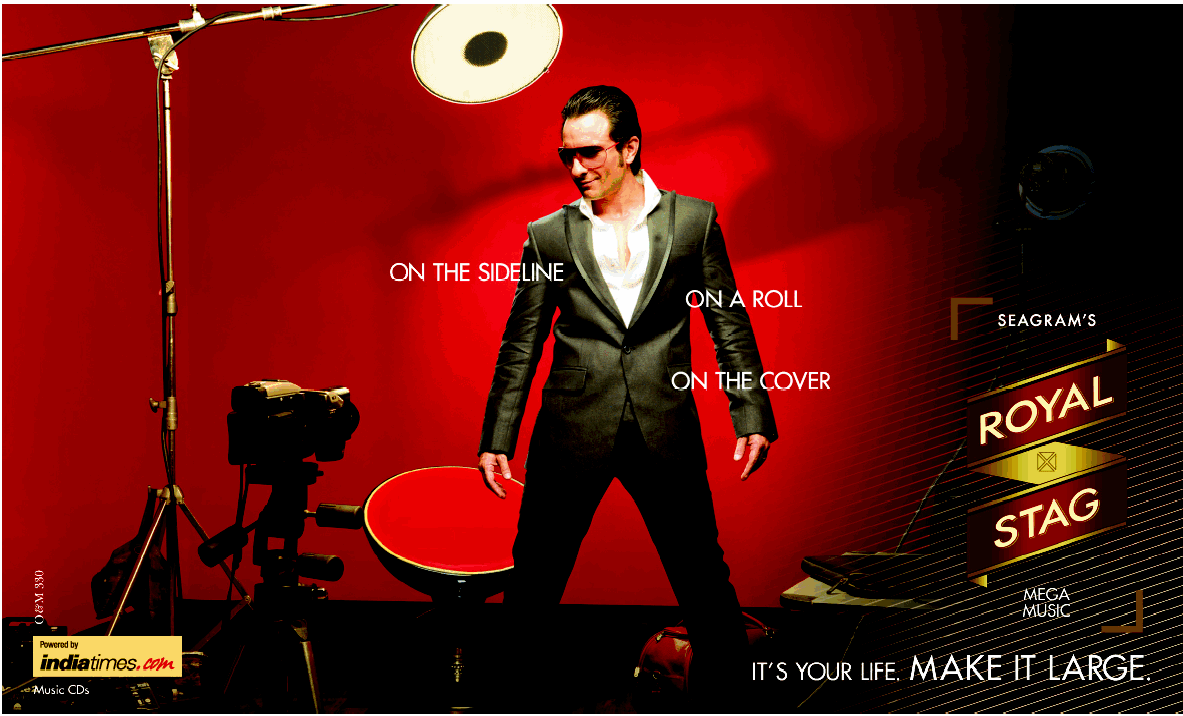
\includegraphics[width=\textwidth]{royalstagad1.png}
\end{figure}

Surveys say that over 80 people out of a 100 understand the actual liquor being
advertised, which means that it is still an effective way of advertising alcohol.

Although currently legal, the government is currently in the process of banning
surrogate advertisements. This is not certain to happen though.

\subsubsection{Alternate Methods of Advertisement}
With the future of surrogate advertising uncertain, some brands have moved to
the event sponsorship and organisation. Examples of this include Kingfisher
sponsoring many teams in the Indian Premier League. Many alcohol brands
have now started sponsoring many glamorous events to spread their name.

\begin{figure}[h!]
	\caption{Royal Stag Music Advert which would commonly be seen on billboards}
	\centering
		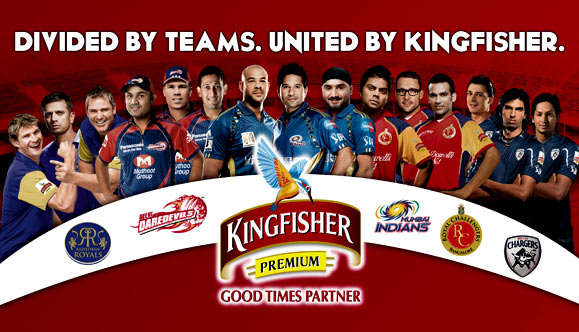
\includegraphics[width=\textwidth]{ipl.jpg}
\end{figure}

\subsection{How We Plan to Advertise Our Product}
\subsubsection{Sponsoring Fashion Shows and Horse Races}
As the microbrewery and cider are new to the city, we would initially have to
spread the name out by spending big. We believe that the best way to do this is
by sponsoring Fashion Shows and Horse Races, as those are the places where we would
get the maximum number of people we are targetting, who are young people, females
and foreigners.
At the events we sponsor, we would get a limited number of bottles of cider produced
so that the people at these events could taste the cider. There would be large banners
around the location which would advertise the microbrewery. We would also hand out
discount coupons at these events which would encourage people to come to the
microbrewery.
By sponsoring these events, we will also obtain the membership data of many
people who would be our potential customers. As we would have phone numbers and
emails, we could send them texts and emails notifying them about the opening of
the microbrewery.

\subsubsection{Initial Discounts on Food and Alcohol}
To attract more people, for the first month of two of the opening of the microbrewery,
we would provide some discounts and offers on some alcohol and food. When people
get to know that they could go to a nice place which is cheaper than the other
places, they would be encouraged to do so. Hopefully, after providing a great first
experience, they would come back in the future.

\subsubsection{Placing Advertisements in the Local Newspapers}
Before opening the microbrewery, we would have to create awareness among the
people of the city that a new microbrewery would be opening up in the city. The
best way to reach to millions of people is by places an advertisement in a popular
newspaper. In the advertisement, we would mention the opening date of the
microbrewery, and also mention the fact that there would be discounts for a short
period of time which would attract more customers.

\subsubsection{Sponsoring Radio Shows}
Along with placing advertisements in newspapers, sponsoring a radio show would reach
out to a large number of people as well. A good time to sponsor a show would be
late night as we would want to target the younger people, who have a tendency to
be awake later than the older population.
\newpage

there is only one other provider of this product hence we see very low competition in this field

Introducing to bars, clubs and hotels in the major cities in India (Delhi, Mumbai, Goa,
Bangalore, Kolkata). Each city would give a different version of the cider, so we would
get a general idea of what the market prefers taste wise.

Low calorie cider?

Need to make other items with the saame brand name, because advertising is limited. Surrogate advertisement

Affiation with a charity? Provide consumers a "feel good" feeling while buying alcohol.

Corruption free

Use of TV and radio. around a billion people listen to the radio, so sponsor the primetime radio
show to spread the name.

Affiliation with the IPL. International market, so easy to introduce Indians to cider.

Cost based pricing vs Price based costing. Cant do competitive analysis, as no cider exists, but compete with
the local beers, etc. Price based costing wins btw.

objective - maximise sales -> how

LTV = (Tn + ATV + LT) - (CoA + CoR)
options which affect LTV

tailor LTV to get maximise value for target customer - guesswork market research
needs to be conducted

how this affects the supply chain
\section{Revenue model}

Initially our main source of revenue would stem from sale of products in the short run once we aim at establishing our brand through adverstising and selling through pubs. Gradually we would like to further increase volume of sales and production and increase revenue through sponsors. In the long run we would like to further increase our product range including different flavours of ciders and gradually streamline our distribution process. This will all result in economies of scale hence reducing cost and added prodict range will increase volume of sales.

\section{Resource, cost and implementation plan}




sources of capital
 % Including headcount plan

\section{Product and systems development plans}
In order to setup a stable and longlasting infrastructure for our business we must take into consideration all the stages and requirements of production. Reaserching our cider recipe constituted the guideline and starting point of a coherent development plan. 

  \subsection{Recipe}
%needs rephrasing
We are planning to operate as a microbrewery producing small volumes of cider. We will start by conducting experiments and testing various recipes to find one which will be most suitable for Indian market. This testing phase significantly reduces our production power as we have to be able to operate quickly and modify recipes according to feedback.\\

We need two types of specialists to operate effectively as microbrewery. These are two initial recipes for our ciders, which we use to estimate cost and quantities of raw ingredients that will be needed. They are most likely to change, and both quantity and exact ingredients will vary depending on the cider recipe development process and the decisions of the brewing master.

		\begin{enumerate}
			\item Ingredients for dry, sparkling cider, 10.5\% abv (per gallon of cider) \\
				\begin{itemize}
					\item Apples - 7kg \\
					\item Yeast (English Cider) - 2g \\
					\item Campden tablets - 1 \\
				\end{itemize}

			\item Ingredients for sweet, sparkling cider,10.5\% abv (per gallon of cider) \\
				\begin{itemize}
					\item Apples - 7kg \\
					\item Yeast (Sweet Mead) - 2g \\
					\item Sugar - 250g \\
					\item Campden tablets - 1 \\
				\end{itemize}
			\end{enumerate}


  \subsection{Licensing}
	To be able to legally operate a brewery in India we are required to obtain a set of licenses. They prove that our that our product is safe for consumption, and that we follow the best standards.\\
	\begin{itemize}
		\item Brewing license \\
		\item Waste water disposal certificate \\
		\item Fabricated equipment quality certificates \\
		\item Water quality testing certificate \\
		\item Quality certificate for beer \\
	\end{itemize}

	\subsection{Space requirements}
When deciding upon our homebase we considered firstly our situation as a new business, with no existing assets or experience, as well as the small scale of our production line. \\

We are aiming to brew \emph{15 gallons per day}. We have already identified the ingredients qunatity requirements per gallon when researching the recipies we will use. Using this information, these are the room size and functionality requirements we identified: \\

  \begin{enumerate}
  \item Ingredients handling room \\
  This room must be easily accessible by our providers and large enough to store a week's worth of ingredients including: \\
    \begin{itemize}
    \item 1500L refrigerator to store 630Kg of apples
    \item 23kg of sugar
    \item yeast, campden tablets
    \end{itemize}
  The room must have a constant supply of water for washing apples and equipment. \\
  The room will operate a weekly pipeline of ingredients storage, however spare space must be available for unforseen situations.\\
  The room size must also allow washing, grating and pressing of apples which implies equipment and staff as detailed in the following sections.

  \item Brewing room \\
  This room must accomodate the two brewing systems for dry and sweet cider: aproximately $2m^3$ each. It must also be able to fit a desk and file cabinet for general office equipment.
  \item Fermenting room \\
  This room will operate a daily pipeline and must be able to accomodate a weeks worth of produce: $4m^3$. It must maintain a constant temperature of aproximately $22^\circ$C for fermentation. We have decided upon this as a good trade-off between quality and speed which are inveresely proportional: a lower fermenting temperature yelds higher quality but requires more time. However this is a specific decision the brewing master must make daily.

  \item Bottling and storage room \\
  This room must accomodate

  \item Maintainance room\\
  This should be a small room for storing cleaning equipment. It should have access or be attached to a staff restroom.
  \end{enumerate}

  \subsection{Equipment}

    \begin{enumerate}
    \item Production equipment
      \begin{itemize}
      \item Apple wash tub
      \item Apple crushing device
      \item Hand cracked cider press: small
      \item Mash tank: 15 gallon
      \item Sparge tank: 15 gallon
      \item Boil Kettle with a false bottom and a siphoning tube
      \item Chill wizzard with a cold water hoze and oxigen pump
      \item Fermenting tank with blow up valves for speedup: 15 gallon
      \item Propane burner
      \end{itemize}

    \item Storage equipment
      \begin{itemize}
      \item 1500L refridgerator for apple storage
      \item freezer for excess and spare apple woat
      \item Fermenting tanks: as mentioned above, in order to host the weekly pipeline, we require 7 15 gallon tanks and spares.
      \item bottles: we are aiming for a production line of 210 bottles daily therefore our weekly requirements is of aproximately 1300 bottles including spares
      \item boxes and lables
      \item shelves or containers ingredients (which come in their own boxes)
      \end{itemize}

    \item General maintainance equipment
      \begin{itemize}
      \item airconditioning system: for the fermentation process
      \item security alarm ans surveillence system
      \item fire detection system
      \item water filtering system
      \item cleaning equipment: \\
        \begin{itemize}
        \item chemical substances (pbw socution, idophor)
        \item cleaning substances (soap, bleach)
        \item blue roll, toilet roll, cloths
        \item bags, bin bags
        \item hozes, gloves, brooms, mops, buckets
        \end{itemize}
      \item office equipment:
        \begin{itemize}
        \item paper and pens
        \item company stamp, files, plastic sleeves, paper punch, envelopes, stapler and spaples, disposable cups, bin
        \item employee register book, visitor register book
        \item company landline telephone
        \item company laptop
        \item tea, coffee, water
        \item first aid kit
        \end{itemize}
      \end{itemize}

    \end{enumerate}

  \subsection{Workforce}  
  \begin{enumerate}
  \item Qualified Brewmaster \\
He has to have previous experience with brewing various types of cider and would probably have to be recruited from a country with cider making traditions (France, England). He would serve as our cider making expert, being able to swiftly operate the equipment and professionally asses the quality of our cider. He must also supervise the general staff activity and behaviour.

  \item Microbiologist
He would serve as an assistant brewmaster, and would be responsible for conducting cider quality control tests, and performing microbiological analysis. He must also verify all the ingredients including the apples, sugar, yeast and water.
It is important to ensure a good quality especially considering the novelty of our product for this market.

  \item Unqualified labour: our microbrewary requires manual labour as described below. These employees must work with the equipment we provide, attend to washing and maintaing it with resposability. Therefore brief training must be considered as a cost. \\ 
  2 workers in charge of apple receival, washing and sorting
  2 workers in charge of apple grating
  2 workers in charge of apple pressing
  1 worker in charge of general cleaning of the area

  \item Security guard \\
On top of general surveillence, he is in charge of verifying employee ids and greeting visitors.
  \end{enumerate}

  \subsection{Contractors}
Whilst most of our equipment contitutes a one time purchase, some of our requirements are constant and imply a contracting a provider.
		\begin{itemize}
		\item Apple supply \\
    Identify a reliable cheap provider: 630kg/week
		\item Water provider \\
		\item Gas and electricity provider \\
    \item Internet and telephone provider
		\item Bottles provider
		\end{itemize}

  \subsection{Risks}
  \begin{enumerate}
  \item human related
    \begin{itemize}
    \item supply : delivery: maybe extra small freezer (2 days worth) 
              : product wuality risk (redundancy)

    \item late pickup : (extra space?)
    \item worker's experience: us, or hire
    \item injuries (insurance, training),  illness (spare trained professional), misbehaviour
    \item security (24h, think key priveleges: already existent)
    \item working conditions: 
    \end{itemize}
  \item equipment related risks
    \begin{itemize}
    \item breaks (replacements) (have backup?)
    \item power cuts (generator backup? - some need: fridge etc.)
    \item water contamination 
    \item moldy apples
    \item run out of storage space (redundant storage)
    \end{itemize}

  \item ethical risks
    \begin{itemize}
    \item working environment
    \item religious employees
    \item local water supply, disposal of waste (donate apple waste)
    \end{itemize}
  \end{enumerate}

\section{Capital requirements}

Since we aim at setting up a microbrewery to start with in Mumbai. We aim at choosing a location frequented by youth.
Hence renting an area in Lower Parel was chosen as this area is frequented alot by young drinkers willing to try new types of alcohol as if known for its night life.
Rent in this area is roughly about Rs.75/sqfoot per month.
As seen in the requirements:
the area of the kitchen would be estimated at: 300 sq/ft
area of the the actual sit out and bar would be about 2500 sq/ft allowing seating for about 60 people along with a nice bar are that would comfortably fit about 150 people.

Further we would require about 80 different types of spirits ranging from vodka to wine. Initially we would start with about 5 bottles each. On consulting a whole-seller this would cost about Rs 3,50,000 to 4,00,000.

The average cost of hiring waitors is about Rs. 1,00,000 a year we would require about 4 bar tenders 2 barbacks 5 waitors and servers.
A good chef being about Rs. 5,00,000 a year.
Along with this nightly security hire costs about Rs 50,000 annually.

We aim at advertising at horse racing events this has a cost of Rs. 5,00,000 though this number is high it has several benefits in doing so:

1) Conduct contests of skill and award prizes to the public to generate interest.
2) Advertise on the CCTV transmission at all centers .
3) Have full rights for on-site branding across the stands.
4) Name the race to suit its preference.
5) Have its CEO / nominee present the trophy.
6) Be entitled to the free use of lawns above a certain value of sponsorship.
7) Arrange for live entertainment at race time or before or after the event.
8) Promote and your brand the race via mailers/press.
9) Have access to the Club's membership data which consists of thousands of potential customers who represent some of the most well off clients in India.
10) Have promotion on the website with links to the lounges webpage.
11) Get coverage on a major television network as these races will be viewed world wide.



\section{Pricing}
We aim at pricing our cider at about Rs.250 which falls in line which most other mid range beer prices. Hence allowing people to try it as an alternative to beer as for a majority of indians it will be viewed in the same lines. Though this is slightly more expensive than other local beers like Kingfisher available at roughly between Rs150 - Rs.200 . But it does provide a level of slight level exclusivity much desired by the growing youth in Mumbai.

All other alcohols will be sold at the rate roughly found in and around similar pubs in the area. Which is usually sold at a mark up of about 350 percent.

Just to give an idea of expected prices we have attached a menu of cafe zoey a very popular and frequented lounge by several drinkers of all ages.

\begin{figure}[h!]
	\caption{Cafe Zoey Menu}
	%\centering
	%	\includegraphics[width=\textwidth]{menu1.jpg}
\end{figure}


\begin{figure}[h!]
	\caption{Cafe Zoey Menu2}
	%\centering
	%	\includegraphics[width=\textwidth]{menu2.jpg}
\end{figure}


\section{Business opportunities and risks}
\section{Pro-forma financial projections}
\section{Risk analysis}

\end{document}
